\documentclass[12pt, titlepage]{article}

\usepackage{booktabs}
\usepackage{tabularx}
\usepackage{hyperref}
\usepackage{graphicx}
\usepackage[normalem]{ulem}
\usepackage[usenames, dvipsnames]{color}
\hypersetup{
    colorlinks,
    citecolor=black,
    filecolor=black,
    linkcolor=red,
    urlcolor=blue
}
\usepackage[round]{natbib}

\title{SE 3XA3: Software Requirements Specification\\DinoDodger}

\author{Team 39, S.R.A Squad
		\\ Shrey Mittal, mittas1
		\\ Razan Abujarad, abujarar
		\\ Zhiwen Yang, yangz18
}

\date{6 October, 2017}

%\input{../Comments}

\begin{document}

\maketitle

\pagenumbering{roman}
\tableofcontents
\listoftables
\listoffigures

\begin{table}[bp]
\caption{\bf Revision History}
\begin{tabularx}{\textwidth}{p{3cm}p{2cm}X}
\toprule {\bf Date} & {\bf Version} & {\bf Notes}\\
\midrule
\date{2017/10/6} & 1.0 & created SRS\\
\date{2017/11/9} & 1.1 & updated Functional Requirements, enumerated non-Functional requirements and Mandated Constraints\\
\date{2017/12/6} & 1.2 & Final Revision (rev1) of SRS. New edits in red ink; discarded text is striked out.\\
\bottomrule
\end{tabularx}
\end{table}

\newpage

\pagenumbering{arabic}

\section{Project Drivers}

\subsection{The Purpose of the Project}
 The purpose of DinoDodger is for the entertainment of the user. As a redevelopment of Chromium's T-Rex Runner, the game involves a virtual character that is continuously running in one direction within a particular landscape. It encounters obstacles in its path that must be overcome by jumping over them, which the character, under the control of the user, can do by pressing \sout{a key} \textcolor{red}{the Spacebar} on the keyboard. \sout{Each step the character takes unharmed by the obstacles increments the number of points accrued, with the intention of the game to score as high as possible as the game progressively becomes more difficult with the speed of the character and the number of obstacles being encountered. The game only terminates once the character comes into contact with an obstacle. For this project, a variety of characters and landscapes each with their intrinsic obstacles and difficulty levels will be provided to the user to choose.} \textcolor{red}{The objective of this game is to accrue as many points as possible, which, initially at zero increment continuously at a particular time interval as long as the character has not intercepted an obstacle in its path. The game progressively gets difficult with the speed of the obstacles coming towards the character marginally increasing at a certain time interval. For the game's implementation of this project, there will be a simple UI provided that would allow a user choose a combination of character and landscape containing the obstacles. The game window will be larger than before, taking up at least 50\% of the screen size.} 

\subsection{The Stakeholders}

\subsubsection{The Client}
The client of this project is Dr. Asghar Bokhari, Professor of SFWRENG 3XA3 in McMaster University

\subsubsection{The Customers}
This project is intended for a single user of an age group 5 and older. 

\subsubsection{Other Stakeholders}
Other stakeholders for this project include the developers of the game, and any other persons who take interest in its future development.

\subsection{Mandated Constraints}
\begin{enumerate}
\item There must be only a single user interacting with the User Interface of this project at one time
\item The User Interface must take up at least 50 percent of the screen of the device.
\item There must be at least three characters and three landscapes available for the user to choose.
\item Project must be completed by December 2017.
\end{enumerate}

\subsection{Naming Conventions and Terminology}
User Interface: The User Interface is a window that will display the game, acting as the visual medium of communication between the program and the user, taking keyboard and cursor inputs wherever necessary and delivering correct output. \\ \\
Character: A character is the virtual player controlled by the user taking the form of various kinds of dinosaurs.\\ \\
Landscape: The landscape is the virtual environment in which the character runs. Examples include desert, tundra, forest etc.\\ \\
Obstacle: An obstacle is any stationary or mobile object within the landscape that inhibits the character’s path or may come into contact with it. These objects are to be overcome. \\ \\
\textcolor{red}{Gameplay: The stage that displays the game with the character and landscape selected and animated, with Points and Highscore being shown. This stage takes user input to get the character to jump.} \\ \\
\textcolor{red}{Points: A numerical representation of the points accrued during gameplay.} \\ \\
\textcolor{red}{Highscore: A numerical representation of the maximum number of points accrued with the current character and landscape settings (i.e.) the user has only chosen to 'Play again'} \\ \\
\textcolor{red}{Game Over: The state following Gameplay upon collision of the Character with an incoming obstacle.} \\ \\
\textcolor{red}{Play Again: Option given in 'Game Over' state allowing user to re-enter Gameplay scene with current settings.} \\ \\
\textcolor{red}{Main Menu: Option given in 'Game Over' state allowing user to return to the main menu of the UI to choose a different combination of character and landscape.} \\ \\
\textcolor{red}{Cactus: An obstacle on the ground} \\ \\
\textcolor{red}{Pteradactyl: An obstacle flying towards the Character at two different heights.} \\ \\


\subsection{Relevant Facts and Assumptions}
\sout{User has already played an equivalent of this game hence there is no necessity to include instructions}
\begin{itemize}
\item{\textcolor{red}{In case the user has not played an equivalent of this game, simple instuctions are provided on what to do. This includes information on which key to press to get the character to jump and instructions to choose a character and landscape.}}
\item{\textcolor{red}{Assuming game is easy to learn, instructions on where and why to use the jump key are not provided.}}
\end{itemize}

\section{Functional Requirements}

\subsection{The Scope of the Work and the Product}
There is minimal scope for this project since there is only a single user intended to use the product at one time. \\ 

\subsubsection{The Context of the Work}
The game motive is to score as high as possible by overcoming obstacles. There is minimal context apart from this.\\

\subsubsection{Work Partitioning}

\begin{itemize}
\item \sout{Razan: User Interface}
\item \sout{Shrey: Main Module that interacts with User Interface to produce output}
\item \sout{Allen: Creation and animation of characters and background}
\end{itemize}

\noindent{Razan}
\begin{itemize}
\item{\textcolor{red}{UI Module}}
\end{itemize}
Shrey
\begin{itemize}
\item{\textcolor{red}{Cactus Module}}
\item{\textcolor{red}{Pteradactyl Module}}
\item{\textcolor{red}{SpriteAnimation Module}}
\item{\textcolor{red}{PointCounter Module}}
\item{\textcolor{red}{Character Module}}
\item{\textcolor{red}{part of PlayScene Module}}
\end{itemize}
Zhiwen
\begin{itemize}
\item{\textcolor{red}{PlayScene Module}}
\end{itemize}


\subsubsection{Individual Product Use Cases}
\begin{figure}
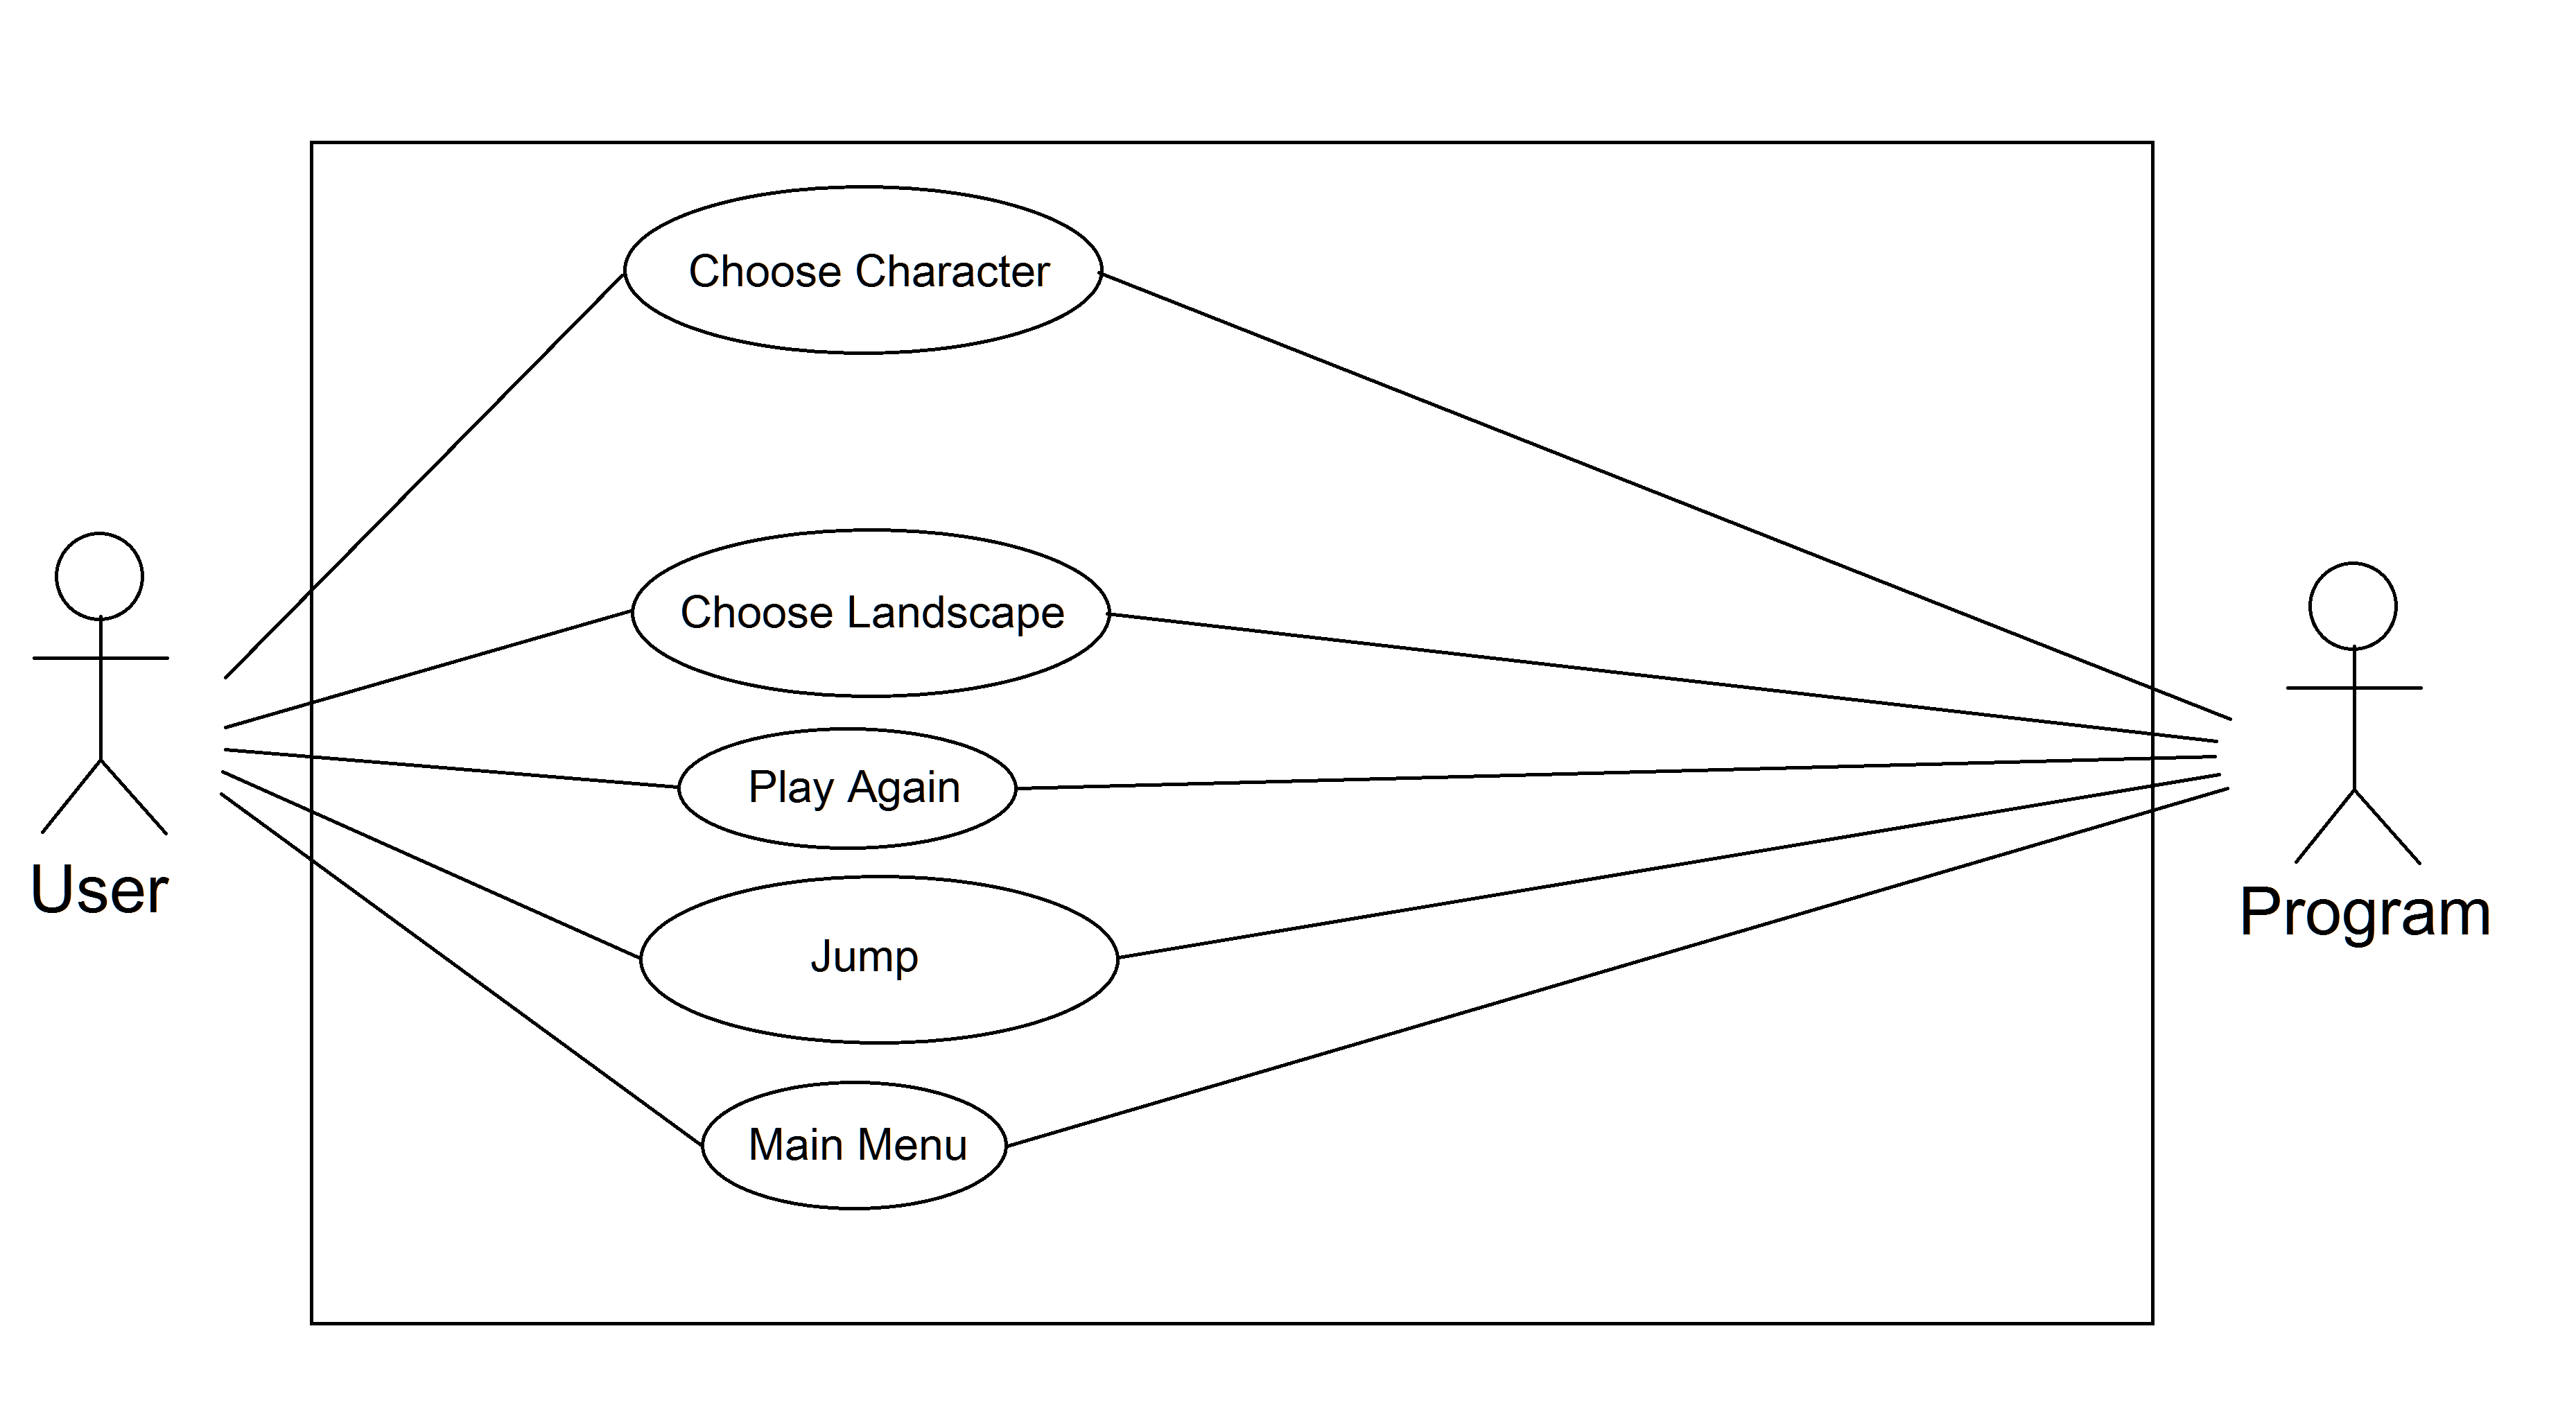
\includegraphics[width = \linewidth]{Use_Case_v1}
\caption{Use Cases Diagram}
\label{Figure 1: Use Cases}
\end{figure}

\subsection{Functional Requirements}
\begin{enumerate}
\item Program must prompt user to select character
\item	Program must prompt user to select landscape
\item	Program must begin game when user \sout{provides key input or uses cursor to click initiatory button.} \textcolor{red}{presses the 'Play' button. Program will transition to the Gameplay stage.}
\item	The user interface must display the animation of a running character from a character’s perspective, meaning the landscape must be animated to be moving relative to the character.
\item	Every time the user presses the \sout{jump} \textcolor{red}{Space} key, the program \sout{responds by showing the character jump from the designated ground level, such that the jump is high enough to overcome the maximum height of obstacles positioned on the ground level, and then land back on the ground. This process should take less than one second to complete} \textcolor{red}{responds by transitioning the Character from its initial y-position along the y-axis to a certain y-position such that cactus obstacles can be overcome and back down to its initial y-position.}
\item	\sout{Game shall terminate when the character comes into contact with an obstacle, meaning there is intersection between the pixels of the character and obstacle.} \textcolor{red}{Upon intersection between character and an obstacle, there is a transition from 'Gameplay' to the 'Game Over' state}
\item	Game shall prompt user to play again or exit, restarting the program or terminating the program based on selection.
\item  During gameplay, program will display the current score and overall highscore \textcolor{red}{on the top right corner of the window}.
\item{\textcolor{red}{When the Space key is pressed and held, the jump transition animation occurs repeatitively until the user releases the key.}}
\item{\textcolor{red}{The program will randomly pick a cactus from a set of cactus images to release them.}}
\item{\textcolor{red}{The program will randomly choose intervals to release Pteradactyls at two different heights}}
\item{\textcolor{red}{The program will randomly choose intervals to release cacti}}
\item{\textcolor{red}{The program will increase the speed of the cacti and the pteradactyls at certain time intervals}}
\item{\textcolor{red}{The highscore is initially 0, and updated only if the value of points exceeds. This happens within the chosen character and landscape settings only}}
\item{\textcolor{red}{Points is always reset to 0 whenever Gameplay stage is entered.}}
\item{\textcolor{red}{In the Game Over stage, the program displays the updated highscore.}}
\item{\textcolor{red}{In the Game Over stage, two options are shown, to 'Play Again', in which current character and landscape choices are maintained and the highscore preserved, and a 'Main Menu' option which brings user back to main menu to choose characters.}}
\item{\textcolor{red}{When program is initially compiled and run, the default character and landscape choices are both grey.}}
\item{\textcolor{red}{Highscore is reset to zero if the user decides to select 'main menu' and select a new character and landscape combination.}}
\item{\textcolor{red}{If user chooses to go back to Main Menu, default character and landscape option does not apply. Same choices are maintained if 'Play' is pressed. }}
\item{\textcolor{red}{The points accrued are updated (incremented) every 200 milliseconds.}}
\item{\textcolor{red}{Pteradactyl must be shown animated.}}


\end{enumerate}
\section{Non-functional Requirements}
The following sections describe the non-functional requirements of DinoDodger.

\subsection{Look and Feel Requirements}
\begin{enumerate}
\item The product shall be comfortable for the user to look at i.e no harsh colour schemes shall be used in the design of the game. \textcolor{red}{The characters and landscapes will have the following color options: grey(original). red, blue}.
\item \sout{The product shall fit into the screen of the device without the user having to readjust any settings of the product.} \textcolor{red}{The UI of the game will use at least 50\% of the screen of the PC. This screen will not be resizable.}
\item Elements of the game shall look cohesive i.e the elements of the game (characters, obstacles) shall have appropriate sizes such that the final product looks well-integrated. 
\end{enumerate}


\subsection{Usability and Humanity Requirements}
\begin{enumerate}
\item The product shall be easy to use by users of a broad age group mostly ages 5+.
\item \sout{The product shall be understandable by users with all language backgrounds}
\item The product shall be used by people without prior training.
\item The product shall be memorable to users i.e users can remember how to use the product at all times.
\item \sout{The product shall retain the highest score obtained by the user.} 
\item \sout{The product shall provide the user a feedback of their current score as well as their highest score at the end of each round} 
\item Users with hearing disabilities shall be able to use the product with ease.
\end{enumerate}

\subsection{Performance Requirements}
\begin{enumerate}
\item  \sout{The product's interface shall have a maximum startup time of 2 seconds after an internet connection becomes unavailable.}
\item \sout{The character element of the product shall response to a screen tap within 0.5 seconds i.e character must jump within 0.5 seconds of user tapping the screen of the phone.}
\item The character element of the product must jump in a time interval equal to the time interval taken to land. 
\item The product shall display the score of the user accurately within 1 point.
\item \sout{The product shall be available 24 hours per day, 365 days per year given an internet connection is absent.}
\item The product shall operate for a period of at least 3 months with minimal maintenance. 
\item The product shall be able to operate continuously for at least 1 hour without crashing or producing an error message to the user.
\end{enumerate}

\subsection{Operational and Environmental Requirements}
\begin{enumerate}
\item \sout{The product shall be used at any location that lacks an internet connection.} 
\item The product shall be used in any weather conditions given the device used to use the product is safe from damage.
\item The product shall be used with any level of light or sound that the device used permits i.e maximum and/or minimum brightness and volume level respectively.
\item \sout{The product must be of a size that is compatible with the device used.} \textcolor{red}{Product will be able to run on Windows and Mac OS systems. This program is not designed for mobiles.}
\item \sout{The product must be installed with the supporting browser and/or application used for browsing the internet.} \textcolor{red}{This program should be easily downloaded and compiled using an executable .jar file or makefile} 
\item \sout{The product must be available for download by the user on any web browser.}
\end{enumerate}

\subsection{Maintainability and Support Requirements}
\begin{enumerate}
\item Additional test cases shall be made for any new features added.
\item The product shall run on any personal computers supporting Java.
\end{enumerate}

\subsection{Security Requirements}
\begin{enumerate}
\item Feedback of the user's score shall be displayed only on the users device. 
\item The user's score shall not be distributed without the consent of the user.
\item The product shall not ask the user for personal information, including name, email, date of birth or banking information.
\end{enumerate}

\subsection{Cultural Requirements}
\begin{enumerate}
\item The product shall not contain any inappropriate symbols. 
\item The product shall not contain any material offensive to religious or ethnic groups.
\end{enumerate}

\subsection{Legal Requirements}
\begin{enumerate}
\item The product shall be ethical and comply with all cyber security laws.
\end{enumerate}

\subsection{Health and Safety Requirements}
\begin{enumerate}
\item \sout{The product shall produce a warning to the user who uses the product continuously for more than 90 minutes. }
\item \sout{The warning shall inform the user of risks  of cramped fingers, eyesight problems and the risk of driving while using the device.}
\end{enumerate}

\section{Project Issues}

\subsection{Open Issues}
\begin{enumerate}
\item The character’s “jump” action performed by pressing spacebar or arrow key
\item 	How complex the animation of the characters will be (simple pixelated or smooth animation)
\item 	What characters and landscapes to create
\item 	Whether this game will include different elevation levels for the character to run on
\item 	If extra features like temporary “power-ups” for the character will be available
\item 	Will audio be included each time an obstacle is overcome or point milestone met
\item 	How points will be calculated, (using time passed or steps taken by the character)
\end{enumerate}

\subsection{Off-the-Shelf Solutions}
- Whether the redevelopment of this project will incorporate ideas from other games like Mario Bros such as different levels and power-ups for the characters \\
- How to evaluate points accrued (number of steps taken, obstacles overcome, time survived) \\

\subsection{New Problems}
- How to enhance difficulty of the game
- What new features to add to the game to improve existing game


\subsection{Tasks}
See use cases diagram in Figure \ref{Figure 1: Use Cases}. 

\subsection{Migration to the New Product}
In order for the intended product-to-be to work, required files must be downloaded and executed. No other steps must be taken. \\

\subsection{Risks}
- Game being hacked and source code being changed.\\

\subsection{Costs}
In order for the intended product-to-be to work, required files must be downloaded and executed. No other steps must be taken.\\

\subsection{User Documentation and Training}
No user licence and prior training is required for this project since it is assumed the project is simple enough for the targeted age group or the user has already been exposed to a game of equivalent difficulty.\\

\subsection{Waiting Room}
As of now all requirements functional and non-functional are to be met by the deadline.\\

\subsection{Ideas for Solutions}
- Designing different characters using MS Paint or obtaining existing images from the Internet \\
- Obtaining designs for landscape and obstacles found within from existing sources or creating new designs using MS Paint or equivalent software \\


\bibliographystyle{plainnat}

\bibliography{SRS}

\end{document}